\chapter{Trabalho Proposto} \label{cap:tp}
%2345678901234567890123456789012345678901234567890123456789012345678901234567890

\todo{dizer em algum lugar antes que conceitos e classes sao considerados os
mesmos}
\todo{dizer em algum lugar tb que relacoes e propriedades sao os mesmos}

\todo{rever no final do cap}
O trabalho visa dois objetivos principais: (i) apoiar o desenvolvimento de
aplicações; (ii) minimizar a dificuldade de configuração existente. O primeiro
objetivo é alcançado com a construção de artefatos de software que leem e
questionam as ontologias via Jason. O segundo objetivo é alcançado pela
criação das ontologias que, além de fazerem o raciocínio, definem um
vocabulário básico a ser conhecido. Por exemplo, um desenvolvedor só
precisa conhecer a ontologia de ambiente proposta para saber\dev{} o que o agente
deve enviar de crenças ou percepções e o que esperar em retorno.

Esse capítulo visa mostrar de maneira organizada a ideia proposta e
desenvolvida. Dessa forma, a primeira seção apresenta a ideia geral do
trabalho sendo proposto. A seguir, a ontologia do modelo afetivo é
apresentada. Em seguida, a ontologia do modelo de percepções é mostrado. Por
fim, a ontologia do modelo de humanos virtuais é discutida e como foi feito a
junção com a mesma.
% cuidar com as palavras: seção, ontologia, modelo

\section{Ontologia Afetiva} \label{cap:tp:oa}

A fundamentação do modelo afetivo sendo utilizado aqui é o proposto por
\citet{ortony1988cse} e encontra-se explicado na seção \ref{cap:eda:mce}
\todo{talvez trocar por uma mais especifica?}. A ontologia proposta tinha
como ideia inicial não utilizar regras, porém como pode ser observado na
Tabela~\ref{tab:oa:geral} foi necessário criar 7 regras para suportar o
raciocínio no nível de indivíduo. Por exemplo, se Fulano avalia que se
relaciona bem com o Ciclano então Fulano tem amigo Ciclano. Note que
o contrario não é necessariamente verdade, o Ciclano pode apenas saber que
conhece o Fulano.

\begin{table}
	\caption{Ontologia proposta com \emph{DL expressivity}: ALCHIN(D).}
	\label{tab:oa:geral}
	\begin{center}
	\begin{tabular}{|c|c|}
	%\begin{tabular}{|p{34mm}|p{50mm}|p{50mm}|}
		\hline
		Descrição & Quantidade \\ \hline
		Classes &  44 		\\ \hline
		Propriedade de Objetos & 14 \\ \hline
		Propriedade de Dados & 12 \\ \hline
		Indivíduos &  0		\\ \hline
		Regras & 7 \\ \hline
	\end{tabular}
	\end{center}
\end{table}

Todos os dados numéricos da ontologia são inteiros. Isso foi feito com a
finalidade de permitir o usuário final normalizar\dev{} o número obtido da
maneira que desejar. Além disso, foi tomada a decisão de não especificar o
domínio de algumas propriedades por causa que isso forçaria um enquadramento
em classes não desejadas. Um indivíduo, por exemplo, com somente a relação
de probabilidade (\emph{hasLikelihood}) seria enquadrado no conceito de
consequência para si (\emph{ConsequenceForSelf}), enquanto o correto seria não
ser concluído nada, isto é, pertencer ao conceito coisa (\emph{Thing}).

\begin{wrapfigure}{r}{0.4\textwidth}
  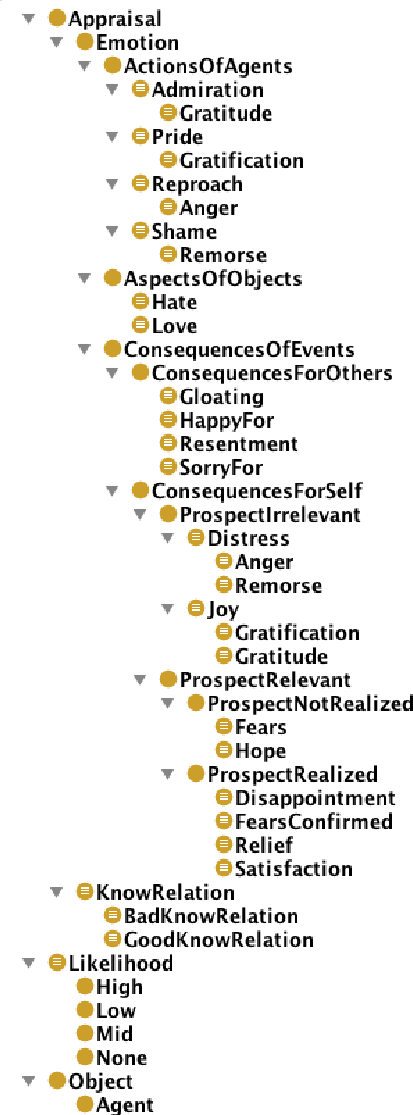
\includegraphics[height=16cm]{figuras/hierarquiaLOCC.png}
  \caption{Taxonomia da ontologia proposta baseado no modelo.}
  \label{fig:tlocc}
\end{wrapfigure}

A estrutura da Figura~\ref{fig:tlocc} será explicada de acordo com a
Figura~\ref{fig:occ_model} (pg. \pageref{fig:occ_model}) da direita para a
esquerda. Para acompanhar o texto é recomendável verificar sempre o que se
esta entre parenteses com a Figura~\ref{fig:tlocc}. As relações encontram-se
disponíveis na Figura~\ref{fig:kplocc}. Dessa forma, o primeiro ramo
é o ramo de aspectos de objetos (\emph{Aspects of Objects}). Ele é o mais
simples dos três que serão abordados e é nele que se encontram emoções do tipo
amor, afeição, repulsa ou ódio.

Essas emoções são relacionadas, de acordo com o modelo, com atratividade e
familiaridade. Entretanto, essas duas relações foram consideradas
equivalentes porque o importante, para o modelo, é quando ambas são positivas
ou ambas são negativas. Assim sendo, uma pode assumir os dois papeis sem
maiores penalidades e simplificando a modelagem. A emoção de ódio
(\emph{Hate}) é modelada como tendo a propriedade de familiaridade
(\emph{hasFamiliarity}) com valores negativos, enquanto o amor (\emph{Love})
tem valoração dessa mesma propriedade positiva. Caso o valor seja zero,
nada pode ser concluído.

Cabe notar que parece estranho uma emoção de amor com um objeto, porém agentes
podem ser vistos como objetos quando se esta avaliando a sua atração. Por
exemplo, Alberto odeia Blueriver ou Millie gosta de rosas vermelhas. Todo
agente (\emph{Agent}) é um objeto (\emph{Object}) e, portanto, o julgamento
de ações não é restrito somente aos agentes.

O segundo ramo é chamado de ações de agentes (\emph{Actions of Agents}), ele
pode ser pensado como um ramo que julga a responsabilidade por uma determinada
ação feita pelo agente sendo julgado. Assim, esse ramo é capaz de gerar 4
emoções: Admiração (\emph{Admiration}), Orgulho (\emph{Pride}),
Vergonha (\emph{Shame}) e Reprovação (\emph{Reproach}). Por exemplo, Millie
possui orgulho por cozinhar ou Jane reprova seu carro novo que esta
apresentando problemas regularmente.

No modelo definido por \citet{ortony1988cse}, as emoções de orgulho e vergonha
podem ser acontecer mesmo quando se esta avaliando ações de outras pessoas.
Por exemplo, Dolares tem vergonha de ter uma mãe que não cozinha. Essa
conclusão no modelo é possível por causa de uma relação que ele propõem
chamada força de unidade cognitiva \footnote{Traduzido literalmente de
\emph{Strength of cognitive unit}.}. Como em nenhum momento na modelagem, ele
dá mais detalhes dessa unidade cognitiva resolveu-se considerar que vergonha e
orgulho são emoções sentidas somente quando o agente esta avaliando a si
mesmo e, dessa forma, o exemplo anterior não é possível.

As emoções que julgam responsabilidade são definidas como tendo uma relação de
julgamento (\emph{hasJudge}) e uma relação que mapeia o valor do julgamento
(\emph{hasJudgeness}) que representa o quanto o agente se desviou do
comportamento esperado, isto é, em casos de aprovação é um valor positivo e em
casos de reprovação é um valor negativo. Todavia, isso ainda não permite
diferenciar a emoção de admiração da emoção de orgulho ou a reprovação da
vergonha. Essa distinção é possível ao se dividir a relação de julgamento com
duas sub-relações: tem auto-julgamento (\emph{hasJudgeMyself}) e tem
julgamento de outro (\emph{hasJudgeOther}).

\begin{figure}
  \centering
  \begin{tabular}{cc}
  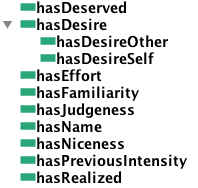
\includegraphics[height=4cm]{figuras/dataProperty-LOCC.png} & 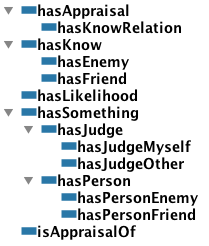
\includegraphics[height=5cm]{figuras/objectProperty-LOCC.png} \\
  (i) Relações de dados & (ii) Relações de Objetos
  \end{tabular}
  \caption{As relações existentes na ontologia proposta.}
  \label{fig:kplocc}
\end{figure}

A utilização de sub-propriedade tem a finalidade de tornar mais fácil as
conclusões do raciocinador. Entretanto, para o usuário pode se tornar
complicado ter que lembrar quando utilizar uma sub-propriedade ou outra.
Assim, foi resolvido deixar o usuário sempre utilizar a relação de julgamento
(\emph{hasJudge}) e via 2 regras inferir se é um auto-julgamento ou o
julgamento de outra pessoa. Para essas regras funcionarem da maneira correta,
o usuário deve declarar que os agentes ou objetos são diferentes. Caso isso
não ocorra, o sistema considera que não há informação para verificar se um
individuo é igual ou diferente que o outro e concluir que não conhece a
resposta.

Por último, o de consequências de eventos (\emph{Consequences of Events})
esta dividido entre consequências para outros (\emph{Consequences for Others})
e para si mesmo (\emph{Consequences for Self}). Todo esse ramo de consequências
de eventos foca na consequência de um evento ou ação realizado por um
determinado agente. Quando se deseja focar em quem fez a ação que originou
a consequência, o usuário deve realizar duas avaliações separadas.

A consequências para outros expressa 4 emoções: felicidade
(\emph{HappyFor}), pena (\emph{SorryFor}), regorizar-se (\emph{Gloating}) e
resentimento (\emph{Resentment}). No modelo, essas emoções dependem: do grau
de desejabilidade nosso para com o outro; do grau de desejabilidade que se
presume que o outro tenha; do grau de merecimento do evento; se nos
relacionamos bem ou não com a pessoa. Na ontologia proposta, a principal
diferença com o modelo original é que consideramos que o grau de
desejabilidade nosso para com o outro e o grau de merecimento do evento são os
mesmos. Dessa forma, se pode utilizar apenas três relações para descrever as
4 emoções.

A relação de merecimento (\emph{hasDeserved}) e relação de desejabilidade
presumida (\emph{hasDesireOther}) são avaliadas de acordo com sua valoração
positiva ou negativa. A terceira relação é a que liga o outro individuo/agente
(\emph{hasPerson}) sendo avaliado. Para se ter o conhecimento de quem esta
julgando é uma pessoa amiga (\emph{GoodKnowRelation}) ou inimiga
(\emph{BadKnowRelation}), esses conceitos foram criados e precisam ser
configurados para cada um dos agentes em questão. O agente pode declarar que
só conhece uma pessoa, que conhece e é um amigo ou que conhece e não gosta
dela (inimiga). Entretanto, quem precisa dessa informação é o conceito de
avaliação quando a relação de pessoa inimiga (\emph{hasPersonEnemy}) ou amiga
(\emph{hasPersonFriend}) precisam ser descobertas.

A consequências para si mesmo do ramo de consequências de eventos é divida
ainda entre consequências de eventos com probabilidade relevante
(\emph{ProspectRelevant}) e irrelevante (\emph{ProspectIrrelevant}). Cabe
salientar que esses dois conceitos se relacionam com probabilidade
(\emph{hasLikelihood}), entretanto enquanto o primeiro conceito se relaciona
com a parte não nula. A outra se relaciona somente com essa.
A classe de probabilidade relevante pode ser dividida ainda entre
possibilidade não realizada (\emph{ProspectNotRealized}) e realizada
(\emph{ProspectRealized}) de acordo com o modelo original.

A classe de possibilidade não realizada (\emph{ProspectNotRealized}) possui as
emoções esperança (\emph{Hope}) e medo (\emph{Fear}). ...

... relevante
	nao realizado
	realizado (probabilidade nao necessaria mais)

... irrelevante 

A um ramo de composicao blablablabal...
%2345678901234567890123456789012345678901234567890123456789012345678901234567890

% Work-a-round
% * Nas consequencias provaveis, efforco-de foi juntado ao tipo de esforço

...

\section{Ontologias do Ambiente} \label{cap:tp:oda}
% de percepcoes virou do ambiente

...

\section{Reutilizando uma Ontologia de Humanos Virtuais} \label{cap:tp:ruodhv}

...
